\section{Push payment}

\begin{figure}[h!]
  \begin{sequencediagram}
    \newinst{payer}{\shortstack{Payer \\
      \\ 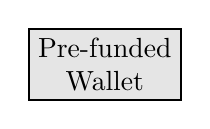
\begin{tikzpicture}
        \node [fill=gray!20,draw=black,thick,align=center] {Pre-funded \\ Wallet};
      \end{tikzpicture}
    }}
    \newinst[2]{exchange}{\shortstack{Taler (exchange) \\
       \\ \begin{tikzpicture}[shape aspect=.5]
        \tikzset{every node/.style={cylinder,shape border rotate=90, draw,fill=gray!25}}
        \node at (1.5,0) {\shortstack{{{\tiny Database}}}};
       \end{tikzpicture}
    }}
    \newinst[2]{payee}{\shortstack{Payee \\
      \\ 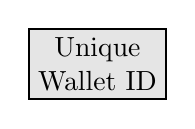
\begin{tikzpicture}
        \node [fill=gray!20,draw=black,thick,align=center] { Unique \\ Wallet ID};
      \end{tikzpicture}
    }}
    \postlevel
    \begin{callself}{payer}{Review push payment fees}{}
    \end{callself}
    \mess[0]{payer}{{Push funds (Coins)}}{exchange}
    \mess[0]{payer}{{Offer payment (e.g. via QR code)}}{payee}
    \begin{callself}{payee}{Review payment offer}{}
    \end{callself}
    \mess[0]{payee}{{Request funds (Wallet ID)}}{exchange}
    \begin{sdblock}{Domestic wallet?}{}
    \begin{callself}{exchange}{Figure~\ref{fig:proc:domestic}}{}
    \end{callself}
    \end{sdblock}
    \begin{sdblock}{KYC/AML required?}{}
    \begin{callself}{exchange}{Figures~\ref{fig:proc:kyc}, \ref{fig:proc:aml}}{}
    \end{callself}
    \end{sdblock}
    \mess[0]{exchange}{{Distribute digital cash}}{payee}
%    \postlevel
    \begin{sdblock}{Payment offer expired?}{}
    \mess[0]{exchange}{{Return funds}}{payer}
    \end{sdblock}

\end{sequencediagram}
  \caption{Interactions between wallets and Taler exchange
    in a push payment.}
  \label{fig:int:push}
\end{figure}
